\section{Моделирование классических антенных решёток}\label{sect:distributions-modeling}

\subsection{Описание программы моделирования и визуализации результатов}\label{sect:distributions-modeling-program}

Моделирование различных антенных решёток проводилось в программном пакете Mathworks MATLAB. Диаграмма, описывающая 
работу написанной программы показана на Рисунке~\ref{fig:array-modeling-program-sch}, 
код программы можно увидеть в Приложении~\ref{appendix:arrays-code-appendix}

\begin{figure}[!ht]
    \centering
    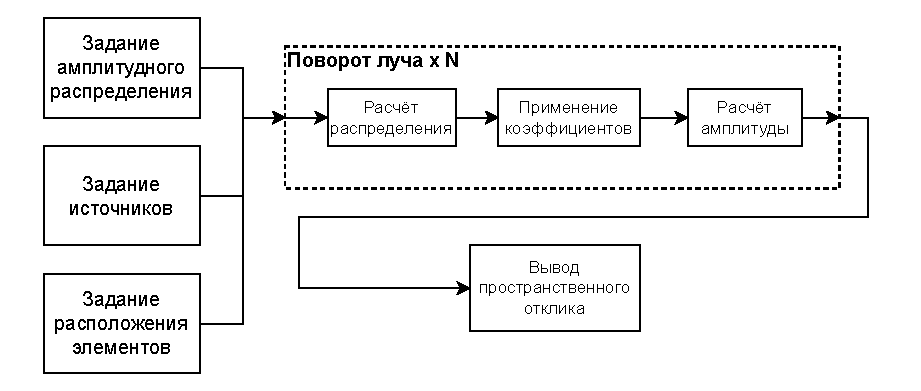
\includegraphics[width=0.8\textwidth,height=0.35\textheight,keepaspectratio]{array-modeling-program-sch}
    \caption{Диаграмма работы программы расчёта}%
    \label{fig:array-modeling-program-sch}
\end{figure}

Процесс работы программы следующий:

\begin{enumerate}
    \item Пользователь вводит амплитуды и направления прихода сигналов
    \item Программа \textit{distribution\_former.m} рассчитывает комплексное распределение на элементах антенны
    \item Промежуточная программа применяет к имеющемуся распределению различные коэффициенты 
    \item Программа \textit{aec\_simulation.m} строит диаграмму направленности и выводит её на экран
\end{enumerate}

В следующих разделах приведены результаты симуляции для антенных решёток, составленных из 24 элементов.

\subsection{Эквидистантная антенная решётка с равномерным распределением амплитуд}

Расположение элементов показано на Рисунке~\ref{fig:equally-spaced-distribution-pos-modeling}. Результаты моделирования отображены на Рисунке~\ref{fig:equally-spaced-distribution-modeling}.

\begin{figure}[!ht]
    \centering
    
\includegraphics[width=0.8\textwidth]{equally-spaced-distribution}
    \caption{Расположение элементов в эквидистантной АР}
    \label{fig:equally-spaced-distribution-pos-modeling}
\end{figure}



\begin{figure}[!ht]
    \centering
    \begin{subfigure}[b]{0.49\textwidth}
        \centering
        \hspace*{-3ex}
        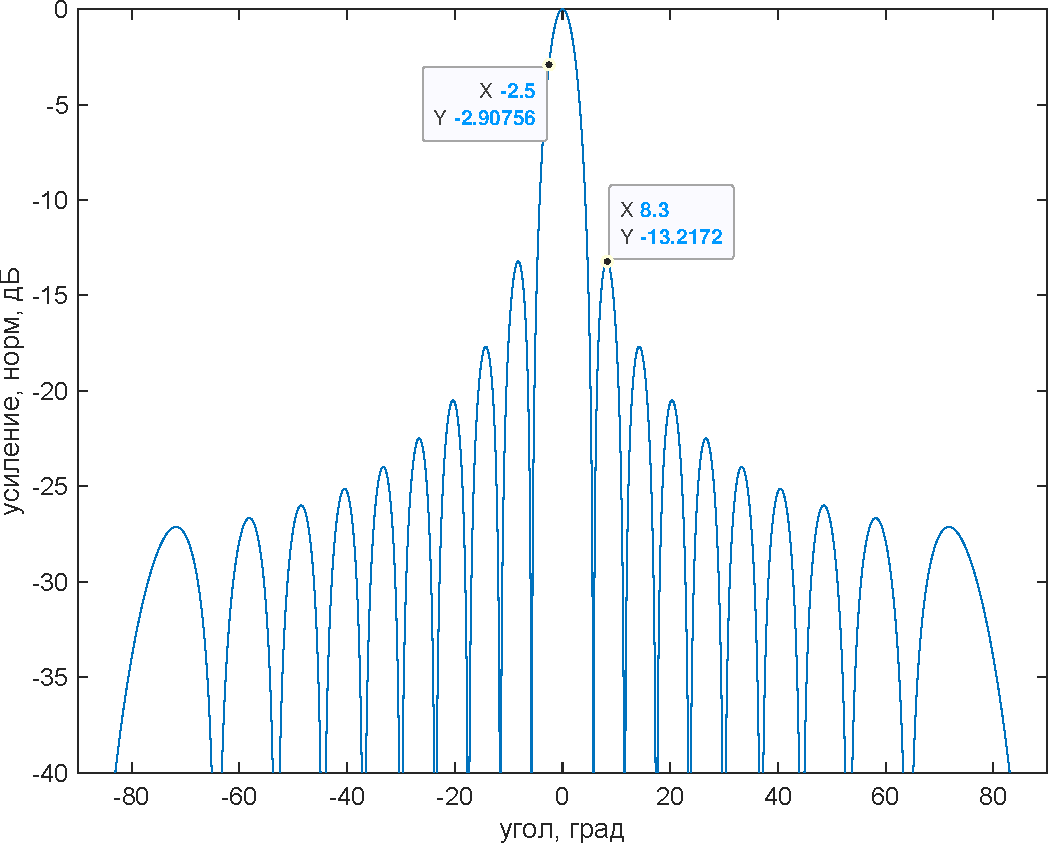
\includegraphics[width=\textwidth]{equally-spaced-distribution-beam-pattern0}
        \caption{}%
    \end{subfigure}
    \hfill
    \begin{subfigure}[b]{0.49\textwidth}
        \centering
        \hspace*{-3ex}
        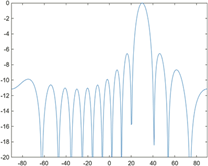
\includegraphics[width=\textwidth]{equally-spaced-distribution-beam-pattern30}
        \caption{}%
    \end{subfigure}
    \caption{%
    Диаграмма направленности АР при направлении главного лепестка на (а) 0 градусов и (б) 30 градусов
    }%
    \label{fig:equally-spaced-distribution-modeling}
\end{figure}

Расстояние между элементами $d=\lambda/2$. Видно, что уровень боковых лепестков составляет $\sim-13$~дБ, 
а ширина главного лепестка равна 5~градусам.

% % %
\subsection{Равномерно спадающее к краям амплитудное распределение}

Расположение элементов показано на Рисунке~\ref{fig:linear-decreasing-amplitude-array-pos}. Результаты моделирования отображены на Рисунке~\ref{fig:linear-decreasing-amplitude-array-modeling}.

\begin{figure}[!ht]
    \centering
    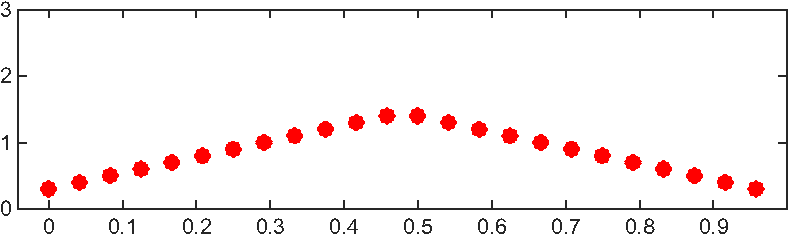
\includegraphics[width=0.8\textwidth]{linear-decreasing-amplitude-array-pos}
    \caption{Расположение элементов в АР}
    \label{fig:linear-decreasing-amplitude-array-pos}
\end{figure}


\begin{figure}[!ht]
    \centering
    \begin{subfigure}[b]{0.49\textwidth}
        \centering
        \hspace*{-3ex}
        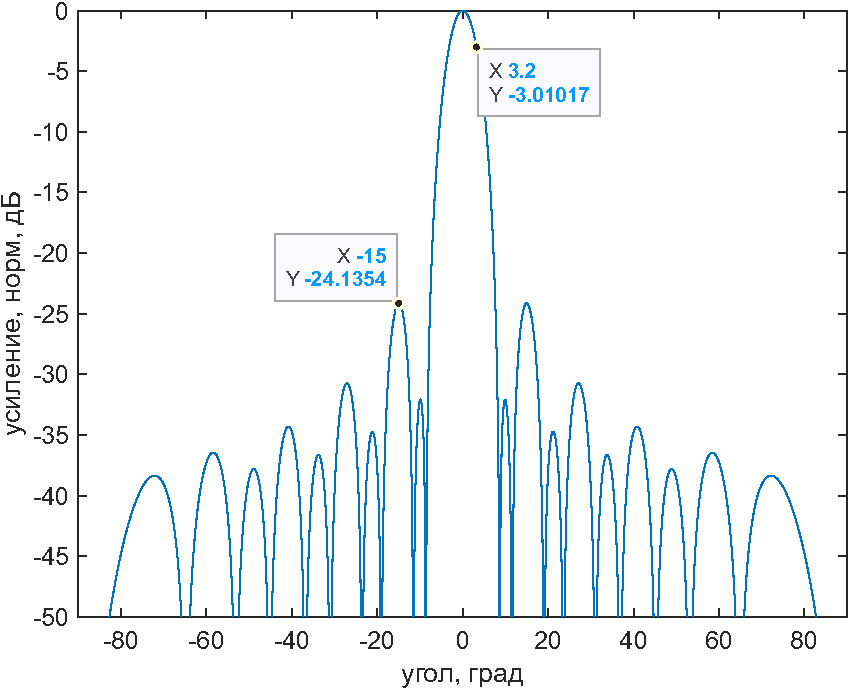
\includegraphics[width=\textwidth]{linear-decreasing-amplitude-array-beam-pattern0}
        \caption{}%
    \end{subfigure}
    \hfill
    \begin{subfigure}[b]{0.49\textwidth}
        \centering
        \hspace*{-3ex}
        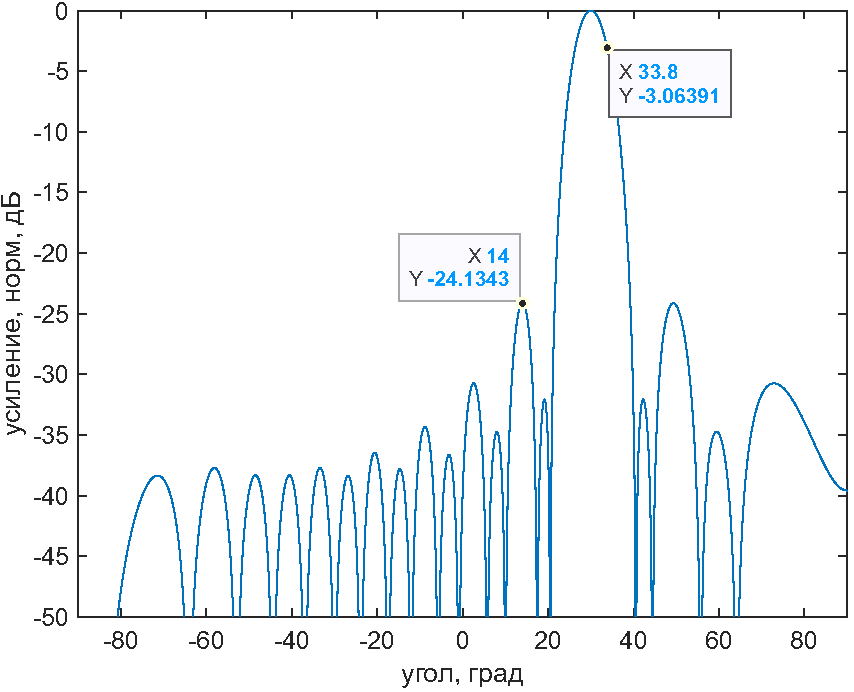
\includegraphics[width=\textwidth]{linear-decreasing-amplitude-array-beam-pattern30}
        \caption{}%
    \end{subfigure}
    \caption{%
    Диаграмма направленности АР при направлении главного лепестка на (а) 0 градусов и (б) 30 градусов
    }%
    \label{fig:linear-decreasing-amplitude-array-modeling}
\end{figure}

Расстояние между элементами $d=\lambda/2$. Видно, что уровень боковых лепестков составляет $\sim-24$~дБ,
что меньше чем при равномерном распределении амплитуд,
а ширина главного лепестка равна $6,2$~градусам, что больше чем при равномерном распределении.

% % %
\subsection{Распределение Дольфа-Чебышева}

Расположение элементов показано на Рисунке~\ref{fig:dolph-tcheby-array-pos}. Результаты моделирования отображены на Рисунке~\ref{fig:dolph-tcheby-array-modeling}.

\begin{figure}[!ht]
    \centering
    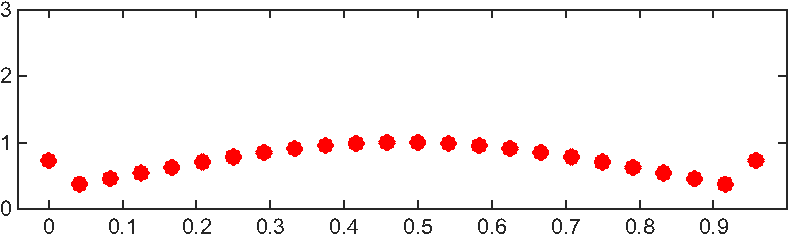
\includegraphics[width=0.8\textwidth]{dolph-tcheby-array-pos}
    \caption{Расположение элементов в АР}
    \label{fig:dolph-tcheby-array-pos}
\end{figure}


\begin{figure}[!ht]
    \centering
    \begin{subfigure}[b]{0.49\textwidth}
        \centering
        \hspace*{-3ex}
        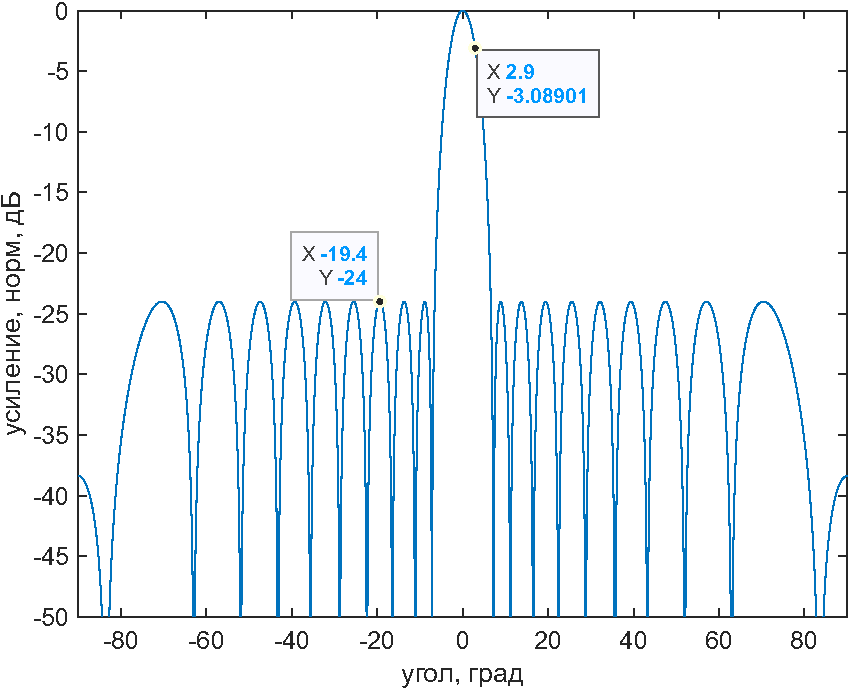
\includegraphics[width=\textwidth]{dolph-tcheby-array-beam-pattern0}
        \caption{}%
    \end{subfigure}
    \hfill
    \begin{subfigure}[b]{0.49\textwidth}
        \centering
        \hspace*{-3ex}
        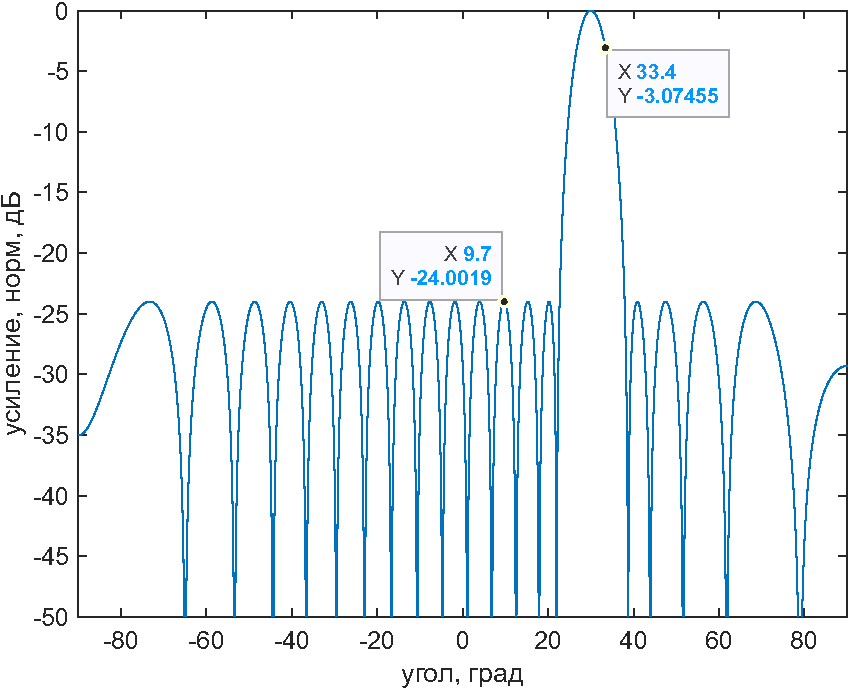
\includegraphics[width=\textwidth]{dolph-tcheby-array-beam-pattern30}
        \caption{}%
    \end{subfigure}
    \caption{%
    Диаграмма направленности АР при направлении главного лепестка на (а) 0 градусов и (б) 30 градусов
    }%
    \label{fig:dolph-tcheby-array-modeling}
\end{figure}

Расстояние между элементами $d=\lambda/2$. Видно, что уровень боковых лепестков составляет $\sim-24$~дБ, 
что меньше чем при равномерном распределении амплитуд, 
а ширина главного лепестка равна $5,8$~градусам, 
что больше чем при равномерном распределении, но меньше чем при равномерно спадающем.

% % %
\subsection{Равномерно возрастающее к краям амплитудное распределение}

Расположение элементов показано на Рисунке~\ref{fig:linear-encreasing-amplitude-array-pos}. Результаты моделирования отображены на Рисунке~\ref{fig:linear-encreasing-amplitude-array-modeling}.

\begin{figure}[!ht]
    \centering
    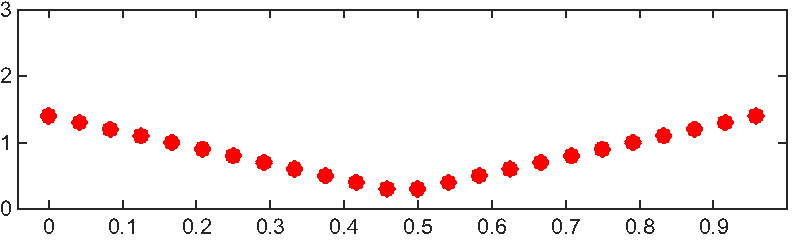
\includegraphics[width=0.8\textwidth]{linear-encreasing-amplitude-array-pos}
    \caption{Расположение элементов в АР}
    \label{fig:linear-encreasing-amplitude-array-pos}
\end{figure}


\begin{figure}[!ht]
    \centering
    \begin{subfigure}[b]{0.49\textwidth}
        \centering
        \hspace*{-3ex}
        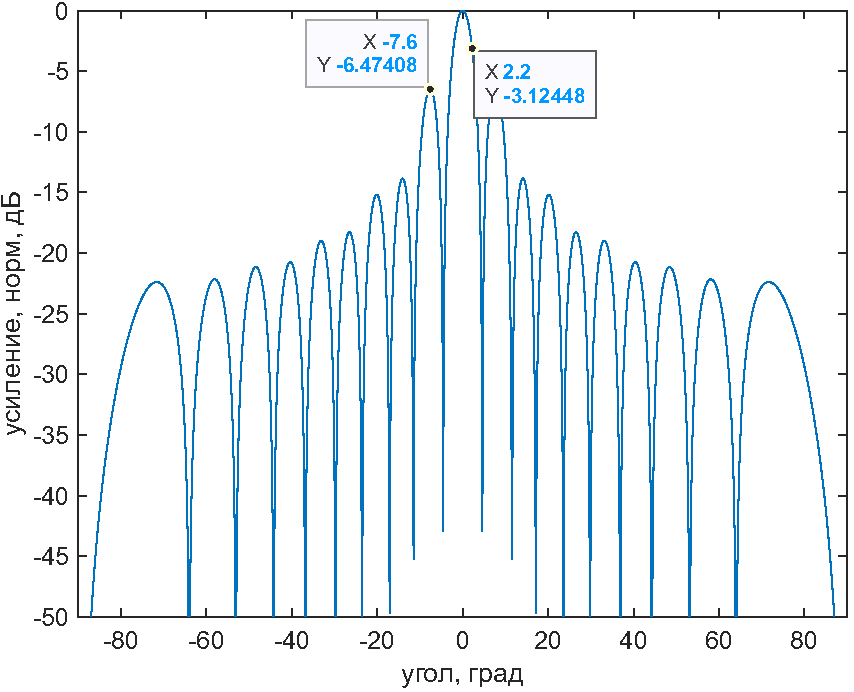
\includegraphics[width=\textwidth]{linear-encreasing-amplitude-array-beam-pattern0}
        \caption{}%
    \end{subfigure}
    \hfill
    \begin{subfigure}[b]{0.49\textwidth}
        \centering
        \hspace*{-3ex}
        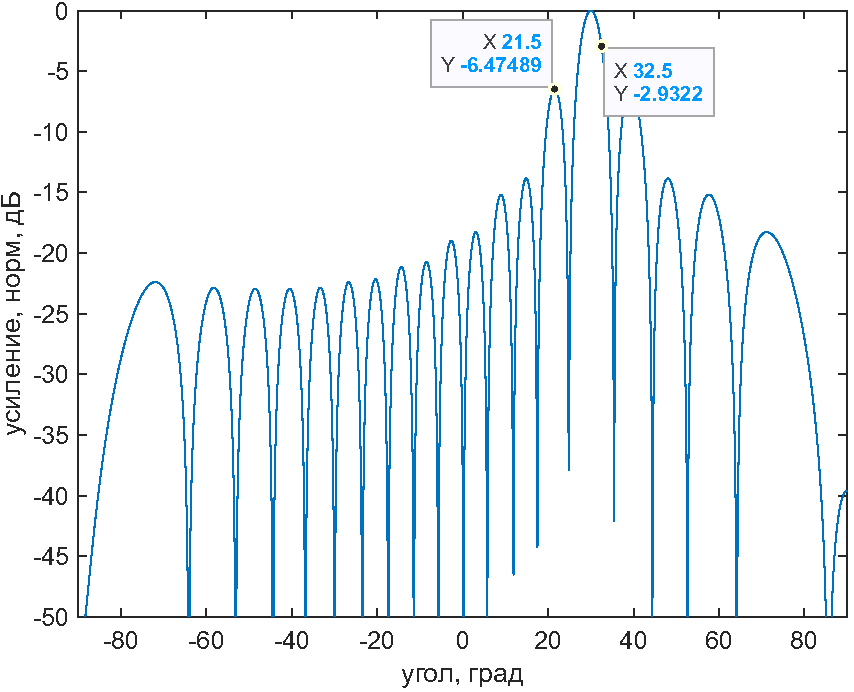
\includegraphics[width=\textwidth]{linear-encreasing-amplitude-array-beam-pattern30}
        \caption{}%
    \end{subfigure}
    \caption{%
    Диаграмма направленности АР при направлении главного лепестка на (а) 0 градусов и (б) 30 градусов
    }%
    \label{fig:linear-encreasing-amplitude-array-modeling}
\end{figure}

Расстояние между элементами $d=\lambda/2$. Видно, что уровень боковых лепестков составляет $\sim-6,4$~дБ, 
что значительно больше чем при равномерном распределении амплитуд, 
однако ширина главного лепестка равна $4,4$~градусам, 
что меньше чем при равномерном распределении.

% % %
\subsection{Расширяющееся к краям геометрическое распределение}

Расположение элементов показано на Рисунке~\ref{fig:side-widing-array-pos}. Результаты моделирования отображены на Рисунке~\ref{fig:side-widing-array-modeling}.

\begin{figure}[!ht]
    \centering
    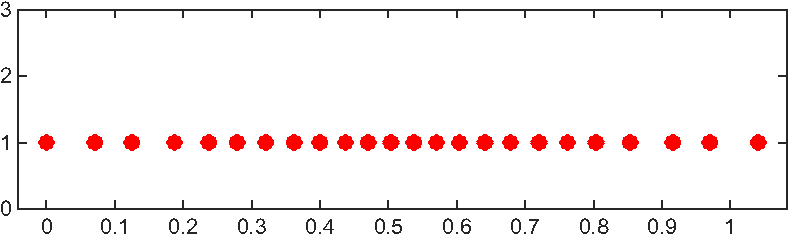
\includegraphics[width=0.8\textwidth]{side-widing-array-pos}
    \caption{Расположение элементов в АР}
    \label{fig:side-widing-array-pos}
\end{figure}


\begin{figure}[!ht]
    \centering
    \begin{subfigure}[b]{0.49\textwidth}
        \centering
        \hspace*{-3ex}
        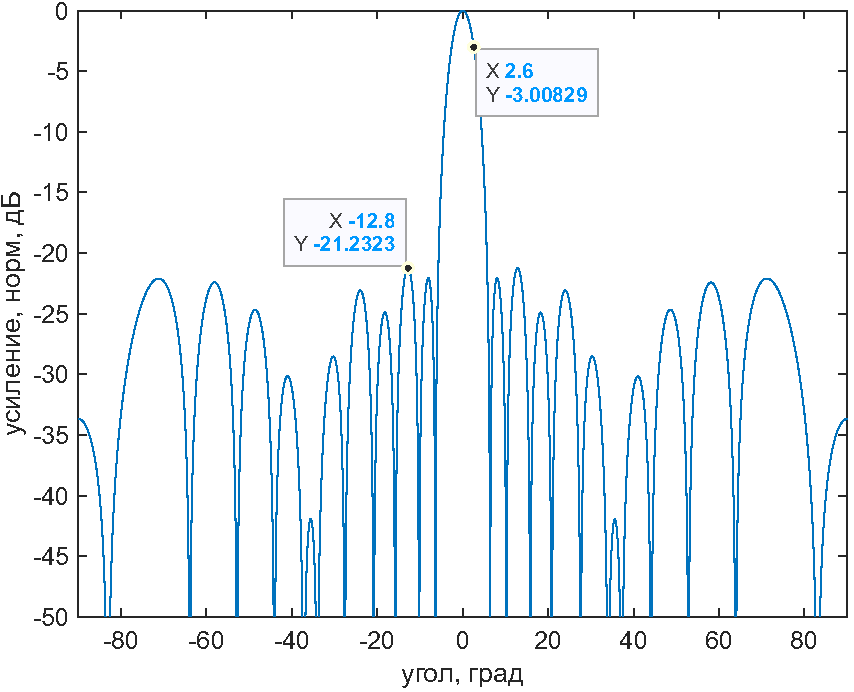
\includegraphics[width=\textwidth]{side-widing-array-beam-pattern0}
        \caption{}%
    \end{subfigure}
    \hfill
    \begin{subfigure}[b]{0.49\textwidth}
        \centering
        \hspace*{-3ex}
        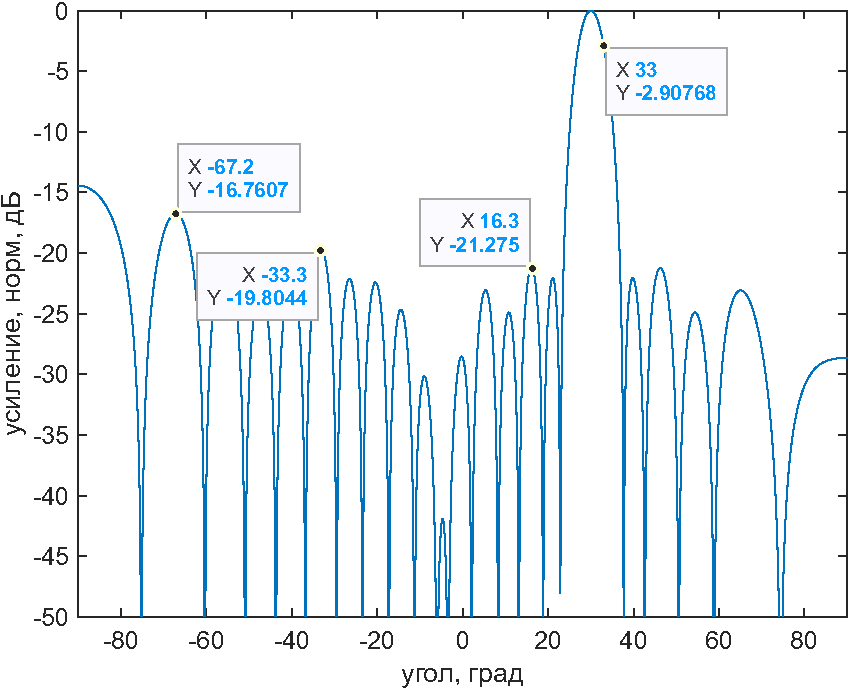
\includegraphics[width=\textwidth]{side-widing-array-beam-pattern30}
        \caption{}%
    \end{subfigure}
    \caption{%
    Диаграмма направленности АР при направлении главного лепестка на (а) 0 градусов и (б) 30 градусов
    }%
    \label{fig:side-widing-array-modeling}
\end{figure}

Расстояние между элементами $d=\lambda/2$. Видно, что уровень боковых лепестков составляет $\sim-21$~дБ, 
что меньше чем в эквидистантной решётке с равномерным распределением амплитуд, 
а ширина главного лепестка равна $5,2$~градусам, 
что немного больше чем при равномерном распределении.

При этом при отклонении на $30$~градусов заметны дифракционные лепестки на уровне $-15$~дБ, в отклонении $-90$ градусов от нормали ($120$~градусов от главного лепестка); а УБЛ составляет $-21 \div -19$~дБ, что также меньше чем при равномерном распределении.

% % %
\subsection{Сужающееся к краям геометрическое распределение}

Расположение элементов показано на Рисунке~\ref{fig:side-narrowing-array-pos}. Результаты моделирования отображены на Рисунке~\ref{fig:side-narrowing-array-modeling}.

\begin{figure}[!ht]
    \centering
    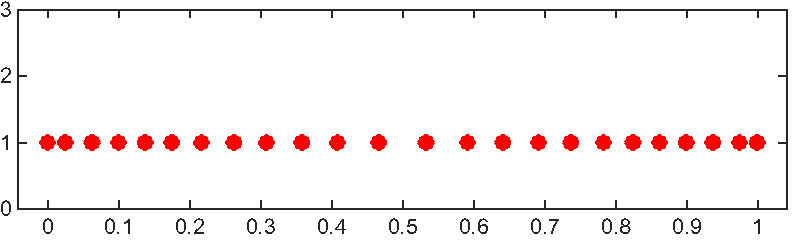
\includegraphics[width=0.8\textwidth]{side-narrowing-array-pos}
    \caption{Расположение элементов в АР}
    \label{fig:side-narrowing-array-pos}
\end{figure}


Расстояние между элементами $d=\lambda/2$. Видно, что уровень боковых лепестков составляет $\sim-10$~дБ, 
что больше чем в эквидистантной решётке с равномерным распределением амплитуд, 
однако ширина главного лепестка равна $4,4$~градусов, 
что меньше чем при равномерном распределении.

\begin{figure}[H]
    \centering
    \begin{subfigure}[b]{0.49\textwidth}
        \centering
        \hspace*{-3ex}
        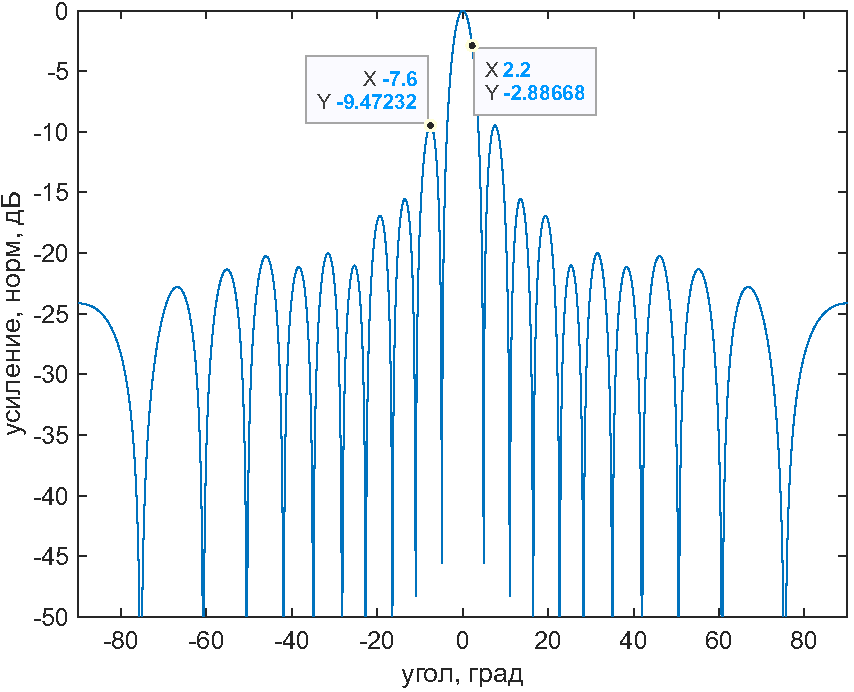
\includegraphics[width=\textwidth]{side-narrowing-array-beam-pattern0}
        \caption{}%
    \end{subfigure}
    \hfill
    \begin{subfigure}[b]{0.49\textwidth}
        \centering
        \hspace*{-3ex}
        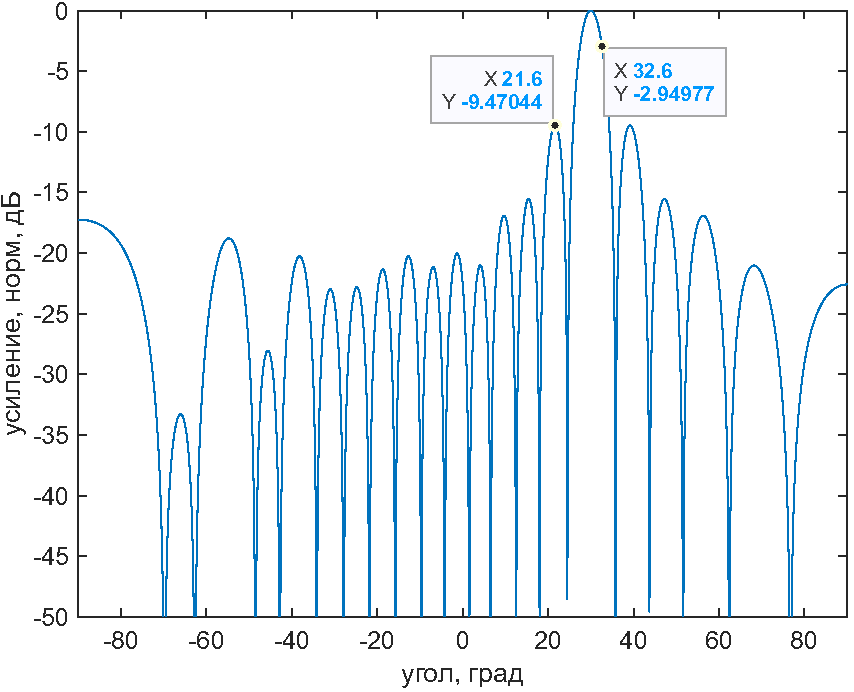
\includegraphics[width=\textwidth]{side-narrowing-array-beam-pattern30}
        \caption{}%
    \end{subfigure}
    \caption{%
    Диаграмма направленности АР при направлении главного лепестка на (а) 0 градусов и (б) 30 градусов
    }%
    \label{fig:side-narrowing-array-modeling}
\end{figure}



% % %
\subsection{Заключение}

По результатам моделирования можно заметить, что концентрация энергии в центре АР уменьшает УБЛ, однако 
увеличивает ширину основного лепестка. В свою очередь уменьшение концентрации энергии в центре АР и увеличение её 
по краям, позволяет немного уменьшить ширину главного лепестка, однако при этом значительно возрастает УБЛ.

Если изменять распределение энергии за счёт изменения положения элементов, то можно получить меньший УБЛ, по 
сравнению с эквидистантными решётками с равным и меньшим количеством элементов, однако при этом будет 
возрастать УДЛ. В то же время можно уменьшать УДЛ по сравнению с эквидистантными решётками, с 
межэлементным расстоянием $d>\lambda/2$, однако при этом, как правило возрастает УБЛ. При этом в обоих случаях, 
ширина главного лепестка остаётся такой же как у эквидистантных решёток либо становится меньше.

Для расчёта распределений в решётках с относительно небольшим количеством элементов удобно применять 
методы, использующие математические приближения, однако для АР с большим числом элементов более выгодным 
становится применение различных генетических алгоритмов либо ручной оптимизации структур с 
изначально нестандартным расположением элементов.

Применение неравномерных распределений позволяет гибко настраивать параметры 
диаграммы направленности антенных решёток. Данный подход имеет следующие преимущества:

\begin{itemize}
    \item Уменьшение УБЛ относительно решёток с равным межэлементным расстоянием
    \item Уменьшение уровня дифракционных лепестков по сравнению с АР с межэлементным расстоянием $d>\lambda/2$
    \item Увеличенная рабочая полоса по сравнению с эквидистантными решётками \cite{andreasen1962linear}
    \item Уменьшение числа элементов по сравнению с 
    эквидистантными решётками со схожими характеристиками направленности
    \item По сравнению с методами, представленными далее, данный подход не требует сложной системы обработки сигнала
\end{itemize}

В то же время данный подход имеет ряд недостатков:

\begin{itemize}
    \item Решётки с неравномерным амплитудным распределением имеют более сложную систему 
    запитки антенных элементов, т.е. более дорогой приемопередающий тракт
    \item Некоторые распределения для неэквидистантных решёток, например вариант 
    из \cite{harrington1961sidelobe}, располагают элементы на расстоянии меньше половины длины волны, 
    из-за чего становится более важно учитывать 
    ЭМ-взаимодействие между элементами \cite{andreasen1962linear}, \cite{ishimaru1962theory}
    \item Разреженные решётки имеют меньший кооэффициент усиления по сравнению с 
    эквидистантными \cite{andreasen1962linear} ввиду меньшего количества антенных элементов
    \item При больших размерах решёток, методы поиска неравномерных геометрических распределений усложняются, 
    а имеющиеся алгоритмы могут давать оптимальные но не наилучшие решения с точки зрения 
    характеристик направленности, хотя и дают выигрыш в стоимости
\end{itemize}